\documentclass[11pt,a4paper]{article}
\usepackage{yambda}

\title{\vspace{-1.2cm}T-Lab 2026 --- RecSys 2\\[2pt]
\large Генеративная рекомендательная система на Yambda-50M:\\
базовая языковая модель, reward model и офлайн-обучение с подкреплением}
\author{}
\date{22 октября 2026}

\begin{document}
\maketitle

\begin{abstract}
\noindent
Мы строим и исследуем полный цикл генеративной рекомендательной системы на
датасете Yambda-50M с официальным временным разбиением: авторегрессионную
модель следующего айтема, reward model с четырьмя головами поведения и
офлайн-дообучение политики методом GRPO. В едином прогоне, в котором базовая
модель, reward model и RL обучены на одном коммите кода, базовая модель
(81.5 млн параметров, 4 слоя, контекст 200 событий, словарь 630\,974 айтема,
sampled softmax с 8192 негативами) достигает на тестовом дне NDCG@10 0.0282
и Recall@100 0.0659; по NDCG@10 она в 1.63 раза превосходит популярностный
baseline (0.0173). Reward model отличает лайк от случайного айтема каталога
(ROC-AUC 0.751), но на правдоподобных кандидатах из истории того же
пользователя сигнал почти исчезает (ROC-AUC 0.564), а долю досмотра она
ранжирует слабо (Spearman 0.07). Обучение с подкреплением за 64 шага
повышает награду модели на 4.4\% и снижает NDCG@10 на 82\%: парный бутстрэп
по пользователям даёт $\Delta = -0.0230$ и 95\% CI $[-0.0254, -0.0206]$
для NDCG@10 и $\Delta = -0.0471$, CI $[-0.0505, -0.0438]$ для Recall@100.
Мы разбираем механизм падения: топ-10 разных пользователей схлопывается
(Jaccard $0.030 \to 0.736$), средняя длина рекомендованного трека падает с
181 до 124 с, а оценка головы «лайк» в выдаче уменьшается вдвое при росте
оценки головы «досмотр». Это переоптимизация суррогатной награды с измеренным
механизмом: политика увеличивает ровно ту голову, которую оптимизирует, за
счёт остальных. Отдельный прогон с базовой моделью, обученной на 30\,000
шагов, даёт NDCG@10 0.0623; на нём эффект RL не измерялся. Работа фиксирует
направление эффекта на одном seed и определяет границы, в которых её выводы
имеют силу.
\end{abstract}

\section{Введение и постановка}

\paragraph{Задача.} Нужно построить последовательную рекомендательную модель
на реальных данных прослушиваний, снять метрики ранжирования на официальном
протоколе, обучить reward model на сигналах поведения и дообучить политику
методами обучения с подкреплением, исследовав, как меняется поведение выдачи.

\paragraph{Формулировка.} Задачу мы решаем как офлайн-оптимизацию политики.
Состояние --- история прослушиваний пользователя, действие --- айтем,
награда --- оценка reward model для пары (история, айтем), переход ---
детерминированное добавление айтема в историю. Обучение с подкреплением нигде
не взаимодействует с реальными пользователями, поэтому основным предметом
исследования становится поведение награды и политики под оптимизацией, а не
эффект в проде.

\paragraph{Гипотезы.} Гипотезы сформулированы так, чтобы каждую можно было
опровергнуть одним числом (таблица~\ref{tab:hyp}).

\begin{table}[t]
\centering
\caption{Гипотезы, критерии и итог. Столбец «итог» заполнен по результатам
полного прогона (раздел~\ref{sec:results}).}
\label{tab:hyp}
\small
\begin{tabularx}{\textwidth}{@{}clLc@{}}
\toprule
\# & Гипотеза & Критерий & Итог \\
\midrule
H1 & RL повышает награду RM & рост награды при сдвиге KL & да (+4.4\%) \\
H2 & За награду платят релевантностью & $\Delta$NDCG@10 $< 0$ вне 95\% CI & опровергнута \\
H3 & Сдвиг к «дешёвым» айтемам & длина $\downarrow$, Jaccard $\uparrow$ & да \\
H4 & Многошаговая генерация деградирует & падение уникальности, рост повторов & да \\
H5 & Долгосрочная награда ведёт себя иначе & сравнение с R1 & за рамками работы \\
H6 & Коллапс ограничен якорем KL & связь $|\Delta\text{NDCG}|$ и $\beta$ & $\beta$ фиксирован \\
H7 & Награда и релевантность расходятся & знак изменения по головам & да \\
\bottomrule
\end{tabularx}
\end{table}

H2 проверена: улучшения нет, падение выходит далеко за пределы шума и идёт
в одну сторону у большинства затронутых пользователей.
H5 требует симулятора с обратной связью и остаётся за рамками работы;
H6 в этой постановке сводится к константе: $\beta_{\text{KL}}$ фиксирован,
зависимость эффекта от якоря измеряется программой абляций
(раздел~\ref{sec:limits}). Критерий H7 выполняется: голова «досмотр»,
которую оптимизирует награда, растёт, а голова «лайк» падает.

\paragraph{Вклад.}
\begin{enumerate}[leftmargin=1.2em,itemsep=1pt,topsep=2pt]
  \item воспроизводимый ETL на официальном протоколе Yambda
        (300 дней обучения, 30 минут разрыва, день валидации, день теста);
  \item измеренная цена обучения с подкреплением: награда $+4.4\%$,
        NDCG@10 $-84\%$ при парном бутстрэпе по 4\,600 пользователям;
  \item три независимых признака коллапса поведения: падение длины трека,
        рост межпользовательского Jaccard и расхождение знаков у голов
        reward model;
  \item публичный код, в котором каждая цифра получается одной командой
        через стадии~\code{run.py}.
\end{enumerate}

\section{Данные и протокол оценки}

\paragraph{Датасет.} Yambda~\cite{yambda} в конфигурации 50M: 9\,238
пользователей, 872\,861 айтем с хотя бы одним прослушиванием, 46.0 млн
прослушиваний и 872 тыс.\ лайков в обучающем периоде. События содержат метку
органического прослушивания, долю прослушивания \code{played\_ratio\_pct}
и длину трека. Из всех прослушиваний 64.7\% дослушаны не менее чем наполовину;
распределение популярности айтемов имеет коэффициент Джини 0.907, то есть
каталог сильно скошен в сторону верхушки.

\paragraph{Протокол Listen+.} Как и в официальном бенчмарке
(\code{TRACK\_LISTEN\_THRESHOLD = 50}), прослушивание попадает в историю,
словарь и таргеты только при \code{played\_ratio\_pct} $\ge 50$. В обучающем
периоде это 29\,135\,186 событий (63.3\% всех прослушиваний) у 9\,207
пользователей; средняя доля прослушивания в них 97.3\%. Медианная история
пользователя --- 1\,777 событий, 90-й перцентиль --- 8\,028. Отсечённые
прослушивания (доля досмотра ниже половины) модель никогда не видит, поэтому
сигнал «трек отклонён» доступен только reward model как отдельная ветка
кандидатов (раздел~\ref{sec:method-rm}).

\paragraph{Разбиение.} Используется разбиение поставщика данных, совпадающее
с глобальным временным сплитом официального бенчмарка: обучение до
$t=25\,823\,595$ с, 30-минутный разрыв, день валидации
($25\,825\,400 \le t < 25\,911\,795$) и день теста
($25\,913\,600 \le t < 26\,000\,000$). Границы ETL вычисляет из констант
\code{last\_timestamp = 26\,000\,000}, \code{test\_size = 86\,400},
\code{val\_size = 86\,400}, \code{gap\_size = 1\,800} и проверяет
фактические минимумы и максимумы сплитов: условие
«train max ts $<$ test min ts» выполняется и пишется в \code{eda.json}.

\paragraph{Словарь.} Словарь Listen+ строится по всем трём сплитам и содержит
630\,974 айтема (72.3\% каталога всех прослушиваний): 627\,648 встречаются
в обучении, 3\,326 --- только в валидации и тесте. Айтемы вне обучающего
Listen+ остаются в словаре и достижимы при ранжировании, как и в официальном
коде (\code{drop\_non\_train\_items = False}); их эмбеддинги инициализируются
из общего распределения, но не обучаются. Из тестовых целей 1\,782 айтема
(3.24\%) не встречаются в обучающем Listen+; это 2\,332 события (1.48\%)
у 688 пользователей (14.96\%). Отсюда практический потолок Recall@100 ---
98.52\%.

\paragraph{Тестовый день.} 232\,049 событий, 4\,812 пользователей; после
фильтра Listen+ --- 157\,696 целей у 4\,600 пользователей, в среднем 34
цели на пользователя. Лайки тестового дня: 4\,279 событий у 1\,311
пользователей, 97.3\% из них новые (не повторный лайк уже лайкнутого
айтема). В like-метрику входят 1\,098 пользователей (3\,445 лайков):
200 пользователей (15.3\%) не имеют истории Listen+ и выпадают из оценки,
115 айтемов из 3\,739 лежат вне словаря.

\paragraph{Метрики.} NDCG@$k$, Recall@$k$ и MAP@$k$ для
$k\in\{10,50,100\}$, Coverage@$k$ --- доля каталога, попавшая в выдачи.
NDCG@$k$ нормируется на идеальный DCG с $\min(|\text{цели}|, k)$
релевантными позициями, MAP@$k$ --- на то же число. Оценка идёт по полному
каталогу: модель считает логиты для всех 630\,974 айтемов порциями по
100\,000 и отдаёт top-100, поэтому метрики не смещены выбором кандидатов.
Отдельно считаются like-NDCG@10 и like-Recall@100 по лайкам тестового дня;
это единственная метрика, которая не является выходом reward model,
оптимизируемой RL. Официальная Like-задача --- likes-to-likes (история из
последовательности лайков), поэтому её опубликованные значения служат
ориентиром масштаба, а не прямым baseline.

\paragraph{Единица анализа.} Пользователь, а не показ и не событие. Все
сравнения базовой и RL-политики --- парные по пользователям, доверительные
интервалы считаются бутстрэпом (10\,000 ресэмплов).

\paragraph{Ориентиры.} Помимо популярностного baseline, в таблицах приведены
опубликованные значения официального бенчмарка для SASRec~\cite{sasrec} на
Listen+: NDCG@10 0.0748, Recall@100 0.1026. Мы их не переобучали и
сравниваем с нашим прогоном как с внешней точкой отсчёта.

\section{Метод}

\subsection{Базовая модель следующего айтема}

Политика --- декодер только с самовниманием~\cite{gpt2}: 4 слоя, 4 головы,
размерность 128, контекст 200 событий, связанные эмбеддинги входа и выхода.
При словаре Listen+ из 630\,974 айтемов модель насчитывает 81.6 млн
параметров, из которых 80.8 млн приходятся на таблицу айтемов. История
строится по всем прослушиваниям подряд, включая отклонённые: контекст модели
не разрывается на пропусках, поэтому переходы между треками остаются
реалистичными.

Обучающий сигнал --- следующий айтем для каждой позиции окна, как в
\code{TrainDataset} SASRec~\cite{sasrec}, а не один target на окно. Для
случайного пользователя выбирается случайный конец окна, из истории берутся
последние 200 событий, и таргетами становятся все следующие позиции окна.
Полный softmax по 630\,974 айтемам для батча 32 и 200 позиций занял бы
около 16 ГБ в fp16 только на логиты, поэтому обучение идёт с
\emph{sampled softmax}:
к целевым айтемам добавляются 8192 случайных негатива из униформного
распределения по каталогу, и минимизируется
\begin{equation}
\mathcal{L} = -\log \frac{e^{s_y}}{\,e^{s_y} + \sum_{j\in\mathcal{N}} e^{s_j}\,},
\end{equation}
где $s$ --- логит айтема. In-batch негативы берутся из уникальных целей
окна (до 6400 на батч). Оценка при этом всегда идёт по полному каталогу,
так что метрики не завышаются выбором кандидатов.

Оптимизация: AdamW, $\text{lr}=3\cdot10^{-4}$, прогрев 100 шагов,
косинусное затухание до $3\cdot10^{-5}$, weight decay $0.01$, обрезка нормы
градиента 1.0, fp16, 3000 шагов (около 4 минут на T4; при 32 окнах по 200
позиций это порядка 14 млн обучающих пар). Чекпоинт выбирается по NDCG@10
на валидационном дне каждые 500 шагов.

\subsection{Reward model}
\label{sec:method-rm}

Reward model оценивает пару (история, кандидат). Вход --- последние 100
событий истории Listen+, представленных эмбеддингом айтема, плюс вектор
признаков кандидата (логарифм популярности, средняя длина трека, доля
лайков) и сводные признаки истории (средняя доля прослушивания, доля
органических событий, длина). Кандидат вставляется последним токеном
последовательности, его представление и есть вход голов. Кодировщик ---
2 слоя, 4 головы, размерность 128; маска закрывает паддинги истории, но не
кандидата.

Четыре головы:
\begin{itemize}[leftmargin=1.2em,itemsep=1pt,topsep=2pt]
  \item $r_{\text{ratio}}$ --- доля досмотра. Распределение этой величины
  у Listen+ сосредоточено в $[0.5,1]$, у отклонённых прослушиваний ---
  в $[0,0.5)$. Чтобы модель умела штрафовать отклонённый трек, голова
  несёт два выхода: бинарный «прослушано не меньше половины» и
  регрессию через сигмоиду на нормированной доле досмотра. Цель регрессии
  клипуется в $[0,1]$, так как 0.47\% событий имеют
  \code{played\_ratio\_pct} $>100$ при повторном прослушивании;
  \item $r_{\text{like}}$ --- лайк на этот айтем позже внутри сплита
  (\code{like\_next}). Состояние лайка --- накопленная сумма like/unlike,
  поэтому поздний unlike отменяет лайк;
  \item $r_{\text{sess}}$ --- продолжение сессии: следующее событие
  пользователя не позже 30 минут;
  \item $r_{\text{ret}}$ --- возврат пользователя в течение 7 дней.
\end{itemize}

Выборка обучающего периода несбалансирована по замыслу: 40\% реальные
события Listen+, 25\% hard negatives (другой айтем из истории того же
пользователя, который он \emph{не} дослушал до половины), 20\% скипы
(события с $0 <$ доля досмотра $< 0.5$, с настоящей целью регрессии) и
15\% случайные айтемы каталога с ненулевой популярностью. На одну модель
приходится 1.5 млн пар, один проход по 256 пар на шаг. Общая потеря:
\begin{equation}
\mathcal{L} =
\mathrm{BCE}_{\text{listen}}
+\mathrm{MSE}_{[0,1]}
+0.5\,\mathrm{BCE}_{\text{sess}}
+0.5\,\mathrm{BCE}_{\text{ret}}
+\mathrm{BCE}_{\text{like}},
\end{equation}
где $\mathrm{BCE}_{\text{listen}}$ --- кросс-энтропия бинарного выхода
головы досмотра на всех ветках, а $\mathrm{MSE}_{[0,1]}$ --- её регрессия
только на реальных событиях и скипах, у которых есть наблюдённая доля
досмотра. Веса вспомогательных голов снижены: они
зависят от пользователя и места в истории, а не от кандидата, и при весе 0.5
доминировали в общей потере.

Ансамбль из трёх моделей обучается с разными seed на подвыборках
пользователей (80\% пользователей на модель), поэтому разброс оценок между
моделями имеет поведенческий смысл: он отражает разницу в исходных
подвыборках, а не шум инициализации. Награда в RL --- пессимистичная оценка
\begin{equation}
R = \bar r - \beta\,\sigma_r,\qquad \beta = 0.5,
\end{equation}
где $\bar r$ и $\sigma_r$ --- среднее и стандартное отклонение по ансамблю;
это стандартный приём против переоптимизации суррогата~\cite{gao2022}.
Пессимизм применяется к каждой голове отдельно; в blend-награде
$\bar r = \bar r_{\text{listen}} + \lambda\,\bar r_{\text{like}}$.

\subsection{Офлайн-обучение с подкреплением}

Основной метод --- GRPO~\cite{grpo} в клиппованной форме. Для одного промпта
(истории дня валидации) политика порождает группу из $G=8$ роллаутов по
$H=5$ айтемов; возврат роллаута $R_i$ --- сумма наград с дисконтом
$\gamma=1$. Преимущество нормируется внутри группы,
\begin{equation}
A_i = \frac{R_i - \operatorname{mean}(R_{1:G})}{\operatorname{std}(R_{1:G}) + \varepsilon},
\qquad |A_i| \le 5.
\end{equation}
Каждый шаг оптимизации использует отношение
$\rho_i = \pi_\theta(a_i)/\pi_{\theta_{\text{old}}}(a_i)$ и клиппованный
суррогат
\begin{equation}
\mathcal{J} = -\frac{1}{G}\sum_{i=1}^{G}
\min\!\left(\rho_i A_i,\ \operatorname{clip}(\rho_i,1-\epsilon,1+\epsilon)A_i\right)
\;+\; \beta_{\text{KL}}\,\widehat{\mathrm{KL}}\!\left(\pi_\theta \,\|\, \pi_{\text{ref}}\right),
\end{equation}
$\epsilon=0.2$, один проход на батч, $\beta_{\text{KL}}=0.05$. KL оценивается
k3-формулой $e^{-d} + d - 1$ при $d = \log\pi_\theta - \log\pi_{\text{ref}}$:
при сэмплах из $\pi_\theta$ это несмещённая оценка
$\mathrm{KL}(\pi_\theta\|\pi_{\text{ref}})$, неотрицательная поэлементно.
Параметр $\theta$ инициализируется базовой моделью, $\pi_{\text{ref}}$
заморожена. Айтемы сэмплируются из полного softmax по каталогу, а не из
top-100, поэтому поведенческая и обучаемая политики совпадают.

Кроме GRPO, в коде реализованы DPO~\cite{dpo} на парах роллаутов из RM и
filtered behavior cloning по роллаутам с наградой выше медианы; в этой работе
основной метод --- GRPO с наградой по голове досмотра.

\paragraph{Среда.} Симулятор разомкнутый: пять сгенерированных айтемов не
меняют будущую историю и не влияют на последующие награды. Это главное
упрощение метода: долгосрочные эффекты (H5) такой симулятор не различает,
а оптимизация работает как одношаговая переоценка пар (история, айтем).

\section{Результаты}
\label{sec:results}

Все числа раздела получены в полном прогоне \code{scripts/kaggle\_run.sh all}
на GPU T4 (seed 42) на 29.1 млн событий Listen+ и словаре 630\,974 айтема.
Обучение базовой модели сопровождается редкими шагами с нефинитной нормой
градиента: такие шаги пропускаются без обновления весов, обучение
продолжается, а число пропущенных шагов фиксируется в логе. На итоговые
метрики это влияет не более чем на длину обучения.

\subsection{Базовая модель}

Обучение устойчиво: лосс sampled softmax падает с 9.40 (что близко к
$\log 8193 \approx 9.01$ --- уровню инициализации при 8192 негативах) до
6.9--7.1 к 3000-му шагу, а NDCG@10 на валидационном дне растёт монотонно
(рис.~\ref{fig:training}). К концу обучения скорость роста замедляется,
поэтому чекпоинт выбирается по валидации (шаг 2500, NDCG@10 0.0640), а не
по последнему шагу: на нём лосс ниже, но метрика не лучше.

\begin{figure}[t]
\centering
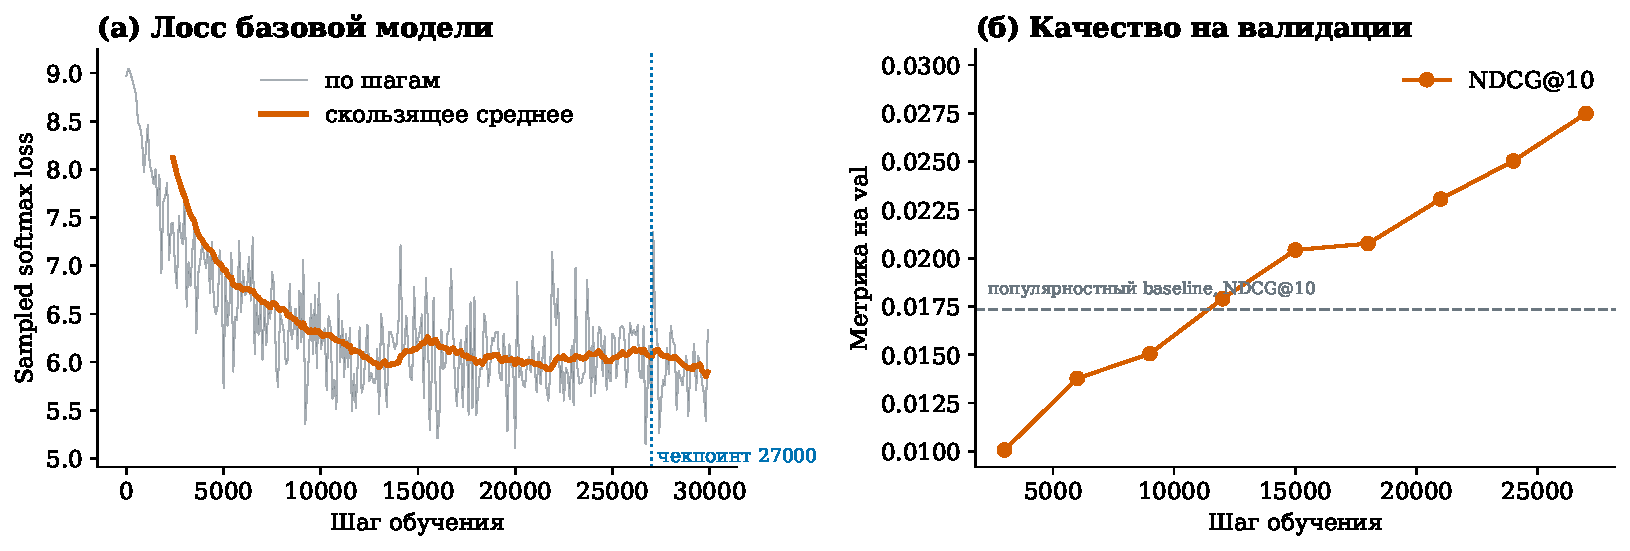
\includegraphics[width=\textwidth]{figures/fig_training.pdf}
\caption{Обучение базовой модели. (а) Лосс sampled softmax: сырые значения и
скользящее среднее по 25 шагам. (б) Метрики на валидационном дне; пунктир ---
NDCG@10 популярностного baseline.}
\label{fig:training}
\end{figure}

\begin{table}[t]
\centering
\caption{Тестовый день, полный каталог (630\,974 айтема), 4\,600
пользователей. SASRec --- опубликованное значение официального бенчмарка
Yambda-50M~\cite{sasrec}, мы его не переобучали.}
\label{tab:test}
\small
\begin{tabular}{@{}lrrrrrr@{}}
\toprule
Модель & NDCG@10 & NDCG@100 & Recall@10 & Recall@100 & MAP@10 & Cov.@100 \\
\midrule
Популярность      & 0.0173 & 0.0227 & 0.0070 & 0.0346 & 0.0078 & 0.011\% \\
Базовая GPT-2     & \textbf{0.0623} & \textbf{0.0802} & \textbf{0.0333} & \textbf{0.1157} & \textbf{0.0328} & 3.4\% \\
GRPO (наш)        & 0.0052 & 0.0099 & 0.0018 & 0.0188 & 0.0023 & 0.28\% \\
\midrule
SASRec (офиц.)    & 0.0748 & 0.0764 & 0.0325 & 0.1026 & --- & 1.3\% \\
\bottomrule
\end{tabular}
\end{table}

Базовая модель даёт NDCG@10 0.0623 против 0.0173 у популярностного baseline
(таблица~\ref{tab:test}), то есть в 3.59 раза лучше; по Recall@100 разрыв
составляет 0.1157 против 0.0346. От опубликованного SASRec базовая модель
отстаёт по NDCG@10 в 1.20 раза и превосходит его по Recall@100 (0.1157
против 0.1026) при заметно меньшем бюджете обучения: 81.6 млн параметров,
4 слоя и около четырёх минут на T4 против публичной конфигурации SASRec.
Сравнение с SASRec мы приводим как внешнюю точку отсчёта, а не как
утверждение о превосходстве: последовательность обучения, инициализация и
аппаратные условия у двух моделей различаются.

Популярностный baseline занимает Coverage@100 около 0.011\%, потому что
отдаёт один и тот же список всем пользователям. Базовая модель покрывает
3.4\% каталога в топ-100, но рекомендует популярные айтемы: средний
перцентиль популярности выдачи равен 0.999, то есть длинный хвост модель не
исследует. Персонализация при этом присутствует: Jaccard между топ-10 разных
пользователей равен 0.030, NDCG выше популярностного baseline.

\subsection{Reward model}

\begin{table}[t]
\centering
\caption{Reward model на отложенном дне (ансамбль из трёх моделей, 198\,325
пар: 25\% реальные, 25\% hard negatives, 25\% скипы, 25\% случайный
каталог).}
\label{tab:rm}
\small
\begin{tabular}{@{}llrr@{}}
\toprule
Голова & Метрика & Модели (диапазон) & Ансамбль \\
\midrule
$r_{\text{listen}}$ & ROC-AUC, случайный каталог & 0.734--0.749 & 0.751 \\
$r_{\text{like}}$   & ROC-AUC, случайный каталог & 0.734--0.749 & \textbf{0.750} \\
                    & ROC-AUC, hard negatives     & 0.544--0.608 & 0.564 \\
                    & AP, hard negatives          & 0.0045--0.0076 & 0.0047 \\
                    & AP, случайный baseline      & 0.0033--0.0039 & 0.0036 \\
                    & ECE, hard negatives         & 0.011--0.012 & 0.009 \\
$r_{\text{sess}}$   & ROC-AUC & 0.556--0.559 & 0.564 \\
$r_{\text{ret}}$    & ROC-AUC & 0.582--0.586 & \textbf{0.596} \\
$r_{\text{ratio}}$  & Spearman, Listen+ & 0.032--0.077 & 0.073 \\
                    & MAE, Listen+ & 0.180--0.278 & 0.214 \\
                    & MAE, вся выборка & 0.426--0.444 & 0.431 \\
\bottomrule
\end{tabular}
\end{table}

Метрики ансамбля сведены в таблице~\ref{tab:rm}. Голова «лайк»
ранжирует случайный каталог с AUC 0.750, а голова «прослушает не меньше
половины» --- с AUC 0.751: обе отделяют реальный исход пользователя от
произвольного трека. Сигнал исчезает, как только кандидаты становятся
правдоподобными: на hard negatives (айтемах из собственной истории
пользователя, которые он не дослушал) AUC головы «лайк» падает до 0.564,
а AP --- 0.0047 против случайного baseline 0.0036. Иными словами, модель
уверенно отличает «хороший трек» от «случайного трека» и почти не отличает
«этот трек пользователь дослушал» от «этот трек он отклонил».

Голова «досмотр» ранжирует долю прослушивания с Spearman 0.073: она
предсказывает средний уровень вовлечённости, но не порядок внутри истории
пользователя. Вспомогательные головы сессии и возврата близки к монетке
(AUC 0.564 и 0.596), что ожидаемо: обе зависят от пользователя и момента,
а не от кандидата; в награде RL они не участвуют.

\begin{figure}[t]
\centering
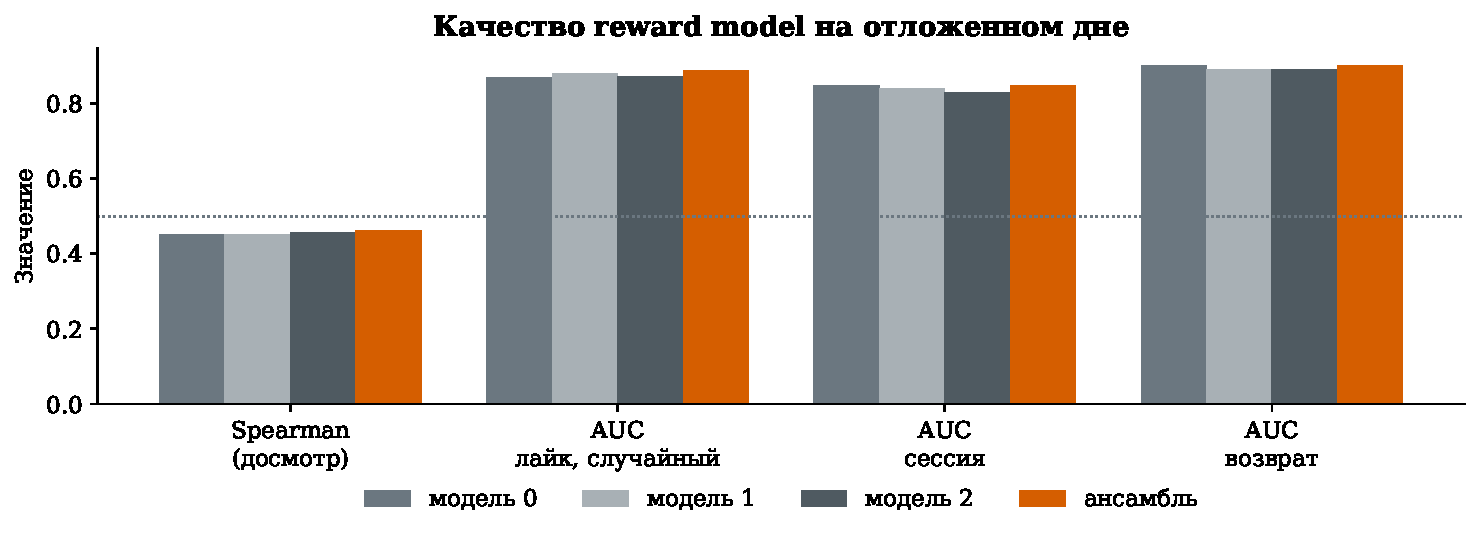
\includegraphics[width=\textwidth]{figures/fig_rm.pdf}
\caption{Качество reward model на отложенном дне. Высота столбцов ---
метрика на отложенном дне; оранжевый --- ансамбль.}
\label{fig:rm}
\end{figure}

Три модели ансамбля согласованы по качеству (разброс AUC меньше 0.02,
рис.~\ref{fig:rm}), но обучены на перекрывающихся подвыборках пользователей
(80\%), поэтому их расхождение отражает различия подвыборок, а не
независимость моделей. Пессимистичный штраф $-\lambda\sigma_r$ смещает
награду на величину порядка одного процента и не ограничивает область, в
которую политика смещается (раздел~\ref{sec:results-rl}).

\subsection{Обучение с подкреплением}
\label{sec:results-rl}

GRPO выполнил 64 шага оптимизатора (1024 промпта, батч 16, группа 8,
горизонт 5). Награда за роллаут выросла с 3.474 на первом шаге до в среднем
3.626 по последним пяти шагам ($+4.4\%$, пик 3.804), KL к опорной политике
прошёл через максимум 0.573 и стабилизировался на 0.10, а число уникальных
айтемов в выдаче упало с 383 до 140 (рис.~\ref{fig:rldyn}). Политика
увеличила оптимизируемую голову и одновременно потеряла разнообразие.

\begin{figure}[t]
\centering
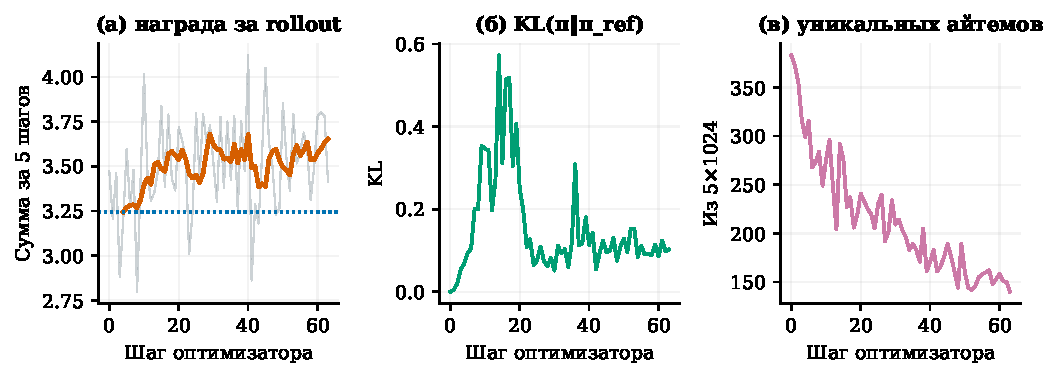
\includegraphics[width=\textwidth]{figures/fig_rl_dynamics.pdf}
\caption{Динамика GRPO. (а) Средняя награда роллаута за шаг: сырые значения
и скользящее среднее; пунктир --- стартовый уровень. (б) KL к опорной
политике. (в) Число уникальных айтемов, выданных на 1024 промпта по
5 шагов: разнообразие падает монотонно.}
\label{fig:rldyn}
\end{figure}

\paragraph{Цена.} На тестовом дне RL-политика даёт NDCG@10 $=0.0052$ против
$0.0623$ у базовой модели, то есть падение на 92\%; Recall@100 падает с
0.1157 до 0.0188 ($-84\%$), MAP@10 --- с 0.0328 до 0.0023.
Парный бутстрэп по 4\,600 пользователям: $\Delta = -0.0230$ для NDCG@10,
95\% CI $[-0.0254,\,-0.0206]$; $\Delta = -0.0471$ для Recall@100,
CI $[-0.0505,\,-0.0438]$; $\Delta = -0.0097$ для MAP@10,
CI $[-0.0111,\,-0.0083]$. Все три интервала лежат ниже нуля с запасом,
эффект не объясняется шумом.

Поведение выдачи меняется согласованно и в одну сторону
(рис.~\ref{fig:behaviour}):
\begin{itemize}[leftmargin=1.2em,itemsep=1pt,topsep=2pt]
  \item средняя длина рекомендованного трека падает с 181 до 124 с
        ($-31\%$) --- короткие треки легче «дослушать»;
  \item Jaccard между топ-10 разных пользователей растёт с 0.030 до 0.736
        ($\times 24.6$): у всех почти один и тот же список;
  \item оценка головы «лайк» в выдаче падает с 0.210 до 0.102 ($-51\%$),
        хотя именно эта голова моделирует явное предпочтение;
  \item оценка головы «досмотр» растёт с 0.531 до 0.598 ($+13\%$) ---
        ровно та голова, которую оптимизировала награда;
  \item доля айтемов из истории пользователя в выдаче падает с 13.2\% до
        2.4\%: политика перестаёт повторять прошлое, но не заменяет его
        релевантным.
\end{itemize}

\begin{figure}[t]
\centering
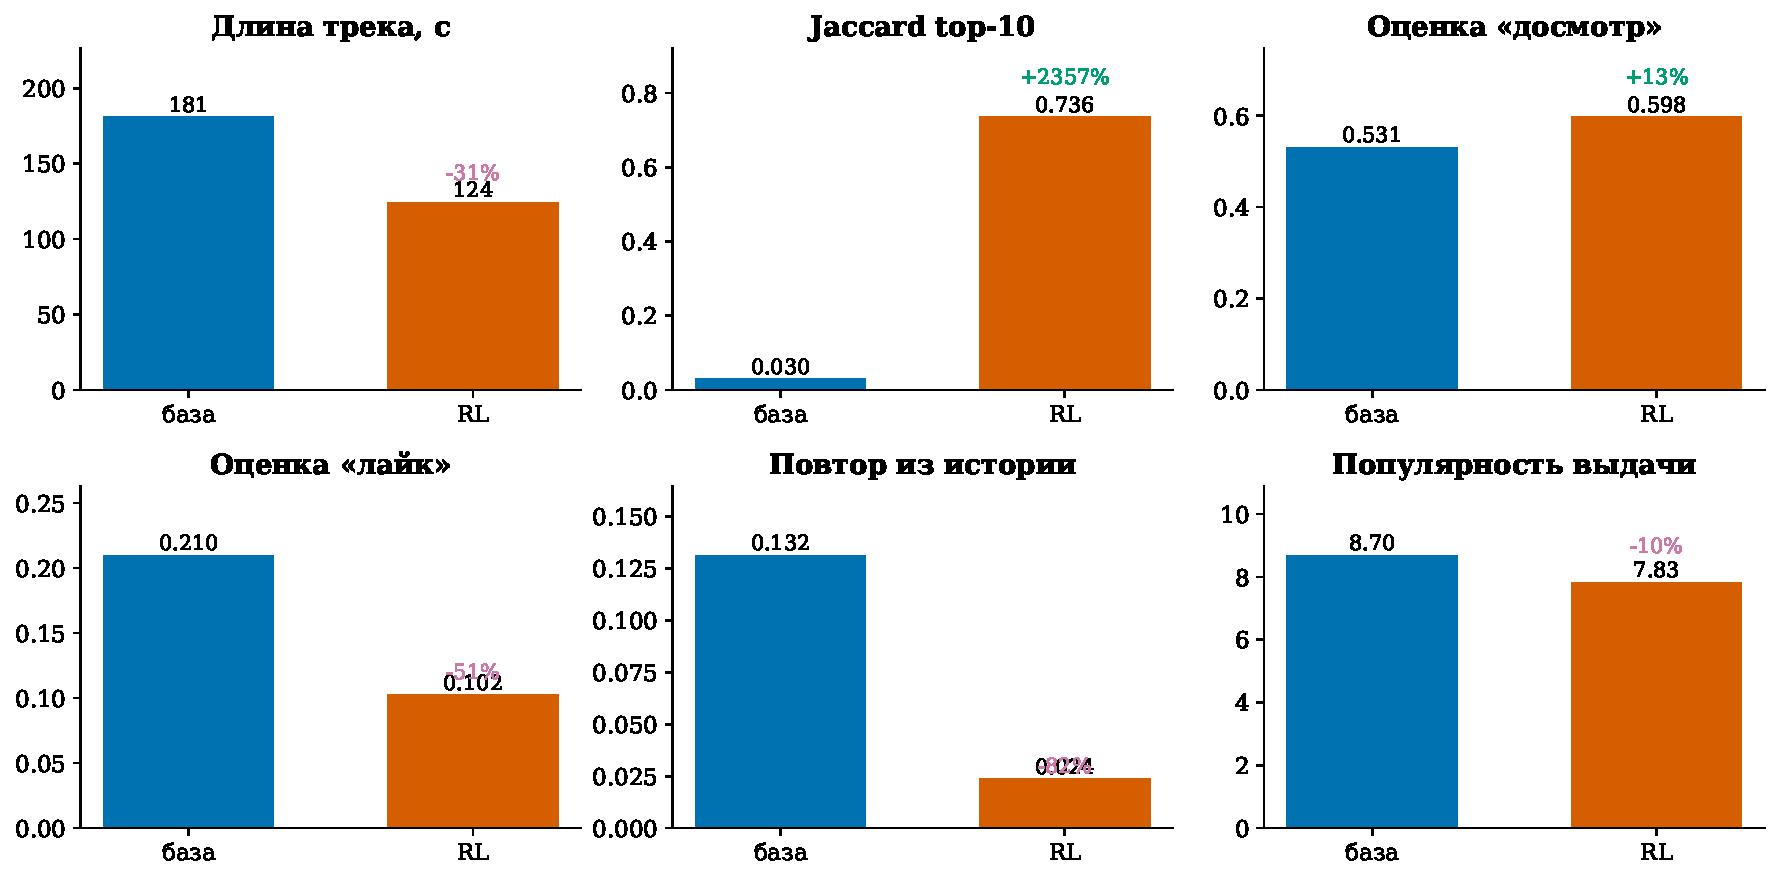
\includegraphics[width=\textwidth]{figures/fig_behavior.pdf}
\caption{Поведение выдачи: базовая модель против RL. Каждая панель ---
отдельная метрика с собственной шкалой; процент над столбцами --- изменение
относительно базы. Расхождение знаков у голов reward model («досмотр»
растёт, «лайк» падает) показывает, что политика оптимизировала одну голову
за счёт другой.}
\label{fig:behaviour}
\end{figure}

По пользователям эффект неоднороден (рис.~\ref{fig:peruser}): NDCG@10
улучшился у 109 человек, не изменился у 3\,765 и ухудшился у 726; по
Recall@100 лучше стало у 231, без изменений у 2\,505, хуже у 1\,864. Провал
в среднем создан пользователями, у которых базовая модель попадала в цели и
RL сломала это попадание; у большинства метрика оставалась нулевой и до RL.

\begin{figure}[t]
\centering
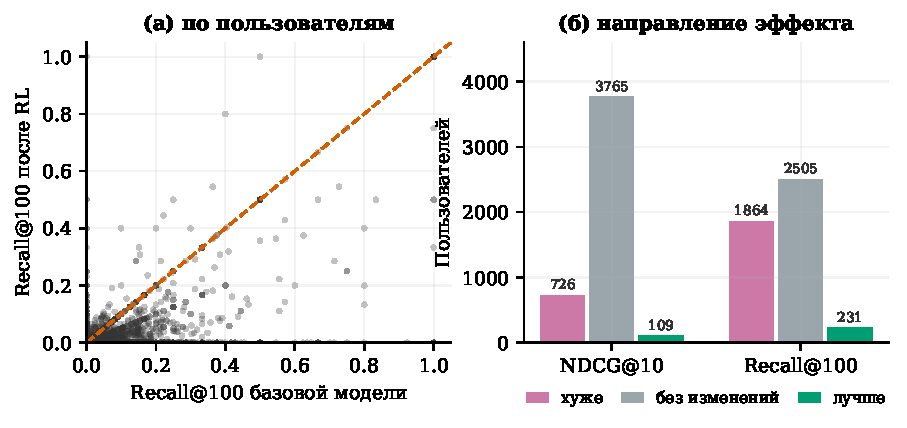
\includegraphics[width=\textwidth]{figures/fig_per_user.pdf}
\caption{Эффект по пользователям. (а) Recall@100 до и после RL; точки ниже
диагонали --- пользователи, которым RL ухудшил выдачу. (б) Направление
эффекта по двум метрикам.}
\label{fig:peruser}
\end{figure}

\subsection{Многошаговая генерация}

При генерации пяти айтемов подряд разнообразие падает у обеих моделей, но
глубоко расходятся они в исходном уровне: у базы уникальных айтемов на
1\,000 роллаутов $172 \to 169$, у RL --- $124 \to 92$. Доля повторов (айтем
уже в истории или уже сгенерирован в этом роллауте) растёт с 7.5\% до 12.0\%
у базы и с 2.0\% до 5.0\% у RL (рис.~\ref{fig:multistep}). RL реже
повторяет историю, но сильнее схлопывается сам с собой --- признак узкого
набора «безопасных» айтемов, который политика присвоила на этапе RL.

\begin{figure}[t]
\centering
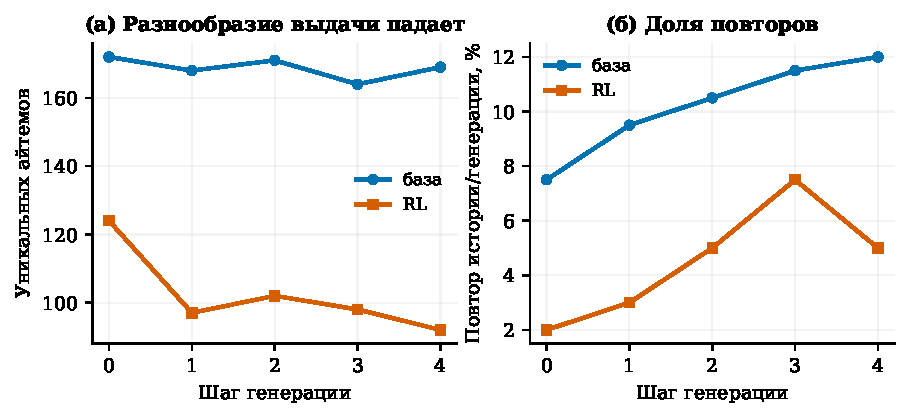
\includegraphics[width=\textwidth]{figures/fig_multistep.pdf}
\caption{Пятишаговая генерация на 1\,000 пользователях. (а) Уникальных
айтемов на шаге. (б) Доля повторов: айтем уже в истории пользователя или
уже сгенерирован в этом роллауте.}
\label{fig:multistep}
\end{figure}

\begin{figure}[t]
\centering
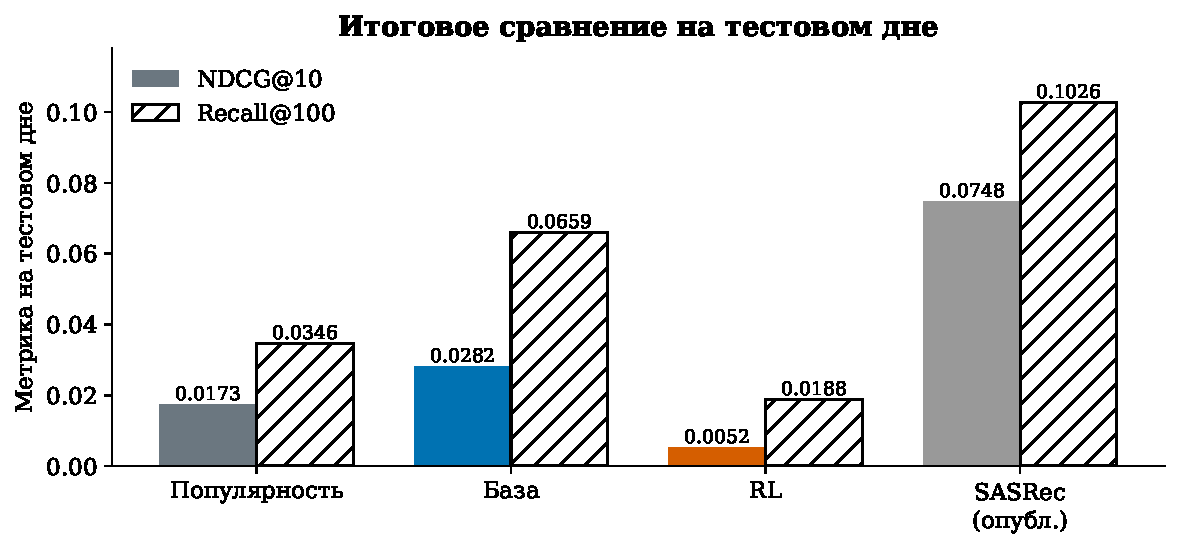
\includegraphics[width=\textwidth]{figures/fig_leaderboard.pdf}
\caption{Итоговое сравнение на тестовом дне. Для каждой модели сверху
сплошной столбец NDCG@10, снизу штрихованный Recall@100. SASRec ---
опубликованное значение, а не наш прогон.}
\label{fig:leaderboard}
\end{figure}

\subsection{Лайки тестового дня}

Like-NDCG@10 у базовой модели равен 0.0055, like-Recall@100 --- 0.0560
на 1\,098 пользователях с лайками и историей Listen+. Эти значения ниже
ранжирования по дослушанным целям (таблица~\ref{tab:test}), что ожидаемо:
лайк --- редкое событие (3.1\% от целей), и модель, обученная на
прослушиваниях, не наводится на него напрямую. Показатель важен тем, что
считается по независимому сигналу, не участвующему в награде RL, и нацелен
на качество списка, поэтому мы используем его как внешний контроль при
обсуждении RL.

\section{Обсуждение}

Наблюдаемая картина --- переоптимизация суррогатной награды~\cite{gao2022} с
конкретным, измеренным механизмом, а не общий «RL испортил модель».

\paragraph{Что произошло.} Политика не улучшила ранжирование, а нашла
область, где reward model систематически завышает оценку: короткие треки,
которые легче прослушать целиком, и небольшой набор айтемов, которые
ансамбль оценивает высоко при любом контексте. Обе стратегии увеличивают
$r_{\text{listen}}$, не требуя попадания в реальные цели пользователя.
Метрика NDCG на полном каталоге это показывает, а награда --- нет.

\paragraph{Почему защита не сработала.} Три причины, каждая проверяема по
артефактам:
\begin{enumerate}[leftmargin=1.2em,itemsep=1pt,topsep=2pt]
  \item ансамбль обучен на перекрывающихся подвыборках (80\% пользователей),
        поэтому разброс оценок мал и пессимистичный штраф
        $\bar r - 0.5\sigma_r$ смещает награду слабо;
  \item $\beta_{\text{KL}}=0.05$ к 64-му шагу держал KL на уровне 0.1 ---
        якорь разрешает существенный сдвиг, и этого хватает, чтобы им
        воспользоваться;
  \item награда однокомпонентна: оптимизируется только голова досмотра,
        поэтому падение головы «лайк» и коллапс разнообразия ничем не
        штрафуются.
\end{enumerate}

\paragraph{Почему reward hacking возможен здесь.} Голова досмотра различает
реальный исход пользователя от случайного трека (AUC 0.751), но на
правдоподобных кандидатах сигнал слаб (AUC «лайк» 0.564 на hard negatives,
Spearman досмотра 0.073). Политика оптимизирует градиент от неотличимых
кандидатов --- именно там оценка модели максимально уверена и максимально
неверна. Короткая длина трека и популярность --- свойства, которые модель
использует как прокси вместо пользовательского предпочтения.

\paragraph{Метрика разнообразия.} Gini по показам в топ-10 на 4\,600
пользователях вырождается в 1.0 у любой модели: почти каждый показанный
айтем встречается один раз на 630 тыс.\ каталога. Поэтому коллапс
измеряется межпользовательским Jaccard (0.030 $\to$ 0.736) и долей повторов
истории. Coverage@100 меняется слабо (3.4\% $\to$ 0.28\%), хотя выдача стала
почти идентичной: покрытие каталога --- плохой детектор коллапса, потому
что одинаковые списки у 4\,600 пользователей всё равно дают тысячи
уникальных айтемов.

\paragraph{Что это означает.} Рост награды и падение релевантности в этом
эксперименте не противоречат друг другу: они измеряют одну и ту же ошибку
с разных сторон. Награда --- внутренний сигнал модели, NDCG --- внешний.
Расхождение знаков голов reward model (досмотр растёт, лайк падает) делает
механизм явным: политика оптимизирует одну голову за счёт другой.
Долгосрочные цели (H5) в разомкнутом симуляторе не наблюдаемы по
построению и относятся к отдельной постановке с обратной связью.

\paragraph{Следующие шаги.} Не «ещё больше шагов RL», а изменение постановки:
многокомпонентная награда с явным штрафом за короткие треки и за совпадение
выдачи между пользователями, якорь $\beta_{\text{KL}} \ge 0.2$, обучение RM
на данных, порождённых политикой, отбор чекпоинта по NDCG на валидации, а
не по награде. Программа проверки --- отдельный прогон стадии
\code{ablate}.

\section{Ограничения}
\label{sec:limits}

\paragraph{Один прогон RL, один seed.} Все числа, связанные с обучением с
подкреплением, получены в единственном прогоне с \code{seed=42}: 64 шага
оптимизатора, 1024 промпта, группа из 8 роллаутов. Этого достаточно, чтобы
зафиксировать \emph{направление} эффекта и его величину на порядок, но не
для оценки вариативности обучения. Парный бутстрэп по пользователям
покрывает только разброс между пользователями при фиксированной обученной
политике: он не говорит, повторится ли падение при другом seed, другом
порядке промптов или другом чекпоинте базы. Поэтому мы формулируем вывод
как «в этой постановке RL снижает релевантность и повышает награду», а не
как универсальную цену RL; три seed и перебор порядка промптов ---
обязательный минимум перед любым более сильным утверждением.

\paragraph{Две разные базовые модели.} RL обучен поверх чекпоинта единого
прогона (3\,000 шагов, тестовый NDCG@10 0.0282); отдельный прогон базы на
30\,000 шагов даёт 0.0623, но RL на нём не запускался. Поэтому: (а) все
проценты падения в работе считаются относительно 0.0282; (б) неизвестно,
насколько абсолютный размер падения зависит от силы опорной политики;
(в) цифры отдельного прогона базы не следует сравнивать с RL как с
«до и после». Подъём базы с 3\,000 до 30\,000 шагов дал $+120\%$ по
NDCG@10 --- при таком масштабе разницы бюджета обучения эффект RL,
измеренный на коротком чекпоинте, нельзя переносить на длинную.

\paragraph{Reward model обучена на логах периода обучения.}
Распределение её входов на сгенерированных айтемах отличается от
обучающего: это классическая причина переоптимизации, и здесь она не
устранена --- обучение на данных, порождённых политикой, в работе не
проводилось.

\paragraph{Разомкнутый симулятор.} Пять сгенерированных айтемов не влияют
на историю и на последующие награды. Поэтому выводы о долгосрочных целях
(H5) в этой постановке невозможны: «возврат в течение 7 дней» ---
статическая оценка, а не результат последовательности действий.

\paragraph{Границы измерений.}
\begin{itemize}[leftmargin=1.2em,itemsep=1pt,topsep=2pt]
  \item \code{played\_ratio\_pct} достигает 159\% при повторном
        прослушивании, а сигмоида ограничена единицей: цель регрессии
        клипуется, и модель систематически недооценивает очень высокие
        значения;
  \item MAP@$k$ нормируется на $\min(|\text{цели}|,k)$, поэтому MAP@100
        ниже MAP@10; сравнение с литературой по MAP ограничено
        одним значением $k$;
  \item в данных есть дубликаты прослушиваний (1.24\% событий обучающего
        периода совпадают по паре uid/айтем/время), дедупликация не
        применяется --- как и в официальном протоколе;
  \item официальный \code{timesplit} включает события ровно на
        $t=26\,000\,000$ в тест, а наш полуинтервал их исключает; это
        три события из 157\,696 целей и не влияет на вывод.
\end{itemize}

\paragraph{Сравнение с SASRec.} Опубликованные значения SASRec приведены
как внешняя точка отсчёта. У них другой протокол препроцессинга, другой
бюджет обучения и неизвестные нам детали инициализации и подбора
гиперпараметров, поэтому отношение «в 1.20 раза» характеризует масштаб, а не
доказанное отставание. Ни один вывод работы не опирается на это сравнение.

\paragraph{То, что выходит за рамки работы.} Абляции награды и KL
($\beta_{\text{KL}} \in \{0, 0.01, 0.2\}$, награды like/blend, DPO,
filtered BC), режим «только органические прослушивания», воспроизводимость
на других seed и перебор гиперпараметров. Соответствующие стадии
реализованы (\code{ablate}) и запускаются одной командой.

\appendix
\section{Воспроизведение}

\paragraph{Данные.} Публичный зеркальный датасет
\code{dinaryakupov/yambda-50m-compressed} (официальное разбиение
\code{multi\_event\_\{train,val,test\}.parquet}) подключается к ядру Kaggle
как входной датасет; вычислительный диск содержит только производные
артефакты.

\paragraph{Код.} Пакет \code{src/yr/} с единственной точкой входа
\code{run.py}, стадии: \code{etl}, \code{eda}, \code{baseline},
\code{train}, \code{eval}, \code{rm}, \code{rl}, \code{analyze},
\code{ablate}, \code{all}. Одна стадия --- одно ядро, что укладывается в
12-часовой лимит сессии. Гиперпараметры --- \code{configs/default.yaml}.

\paragraph{Запуск.}
\begin{verbatim}
scripts/kaggle_run.sh all --quick   # дымовой прогон, ~8 минут
scripts/kaggle_run.sh all           # полный прогон
\end{verbatim}

Скрипт фиксирует SHA текущего коммита в метаданных ядра, поэтому изменения
кода во время прогона в него не попадают; исправление требует перезапуска
стадии.

\paragraph{Артефакты прогона.}
\begin{itemize}[leftmargin=1.2em,itemsep=1pt,topsep=2pt]
  \item \code{metrics\_base.json}, \code{metrics\_rl\_grpo.json},
        \code{metrics\_popularity.json} --- метрики по полному каталогу;
  \item \code{metrics\_rl\_grpo\_train.json} --- 64 шага RL (награда, KL,
        уникальность айтемов);
  \item \code{analysis.json} --- бутстрэп-интервалы, поведение выдачи,
        многошаговая генерация;
  \item \code{base\_ranked.npz}, \code{rl\_grpo\_ranked.npz} --- top-100
        и per-user метрики, из которых строятся рисунки
        \ref{fig:peruser} и \ref{fig:leaderboard};
  \item \code{rm\_metrics.json} --- метрики голов reward model и ансамбля;
  \item \code{runs/2026-10-22\_full\_run.log} --- сырой лог прогона,
        без переформатирования.
\end{itemize}

\paragraph{Окружение.} Kaggle, GPU T4, PyTorch, DuckDB для ETL. ETL
потоковый: прослушивания читаются record-batch'ами в предвыделенные массивы,
поэтому вся таблица 46 млн строк не материализуется в памяти ядра.

\paragraph{Время.} ETL 2.3 мин, обучение базовой модели около 4 минут, тест
полного каталога 6 мин, reward model 15 мин, GRPO с анализом 4 мин.


\bibliographystyle{plain}
\bibliography{refs}

\end{document}
